\section{Conceptual Framework}
\label{sec: design}

\subsection{Concept}

\begin{figure}
    \centering
    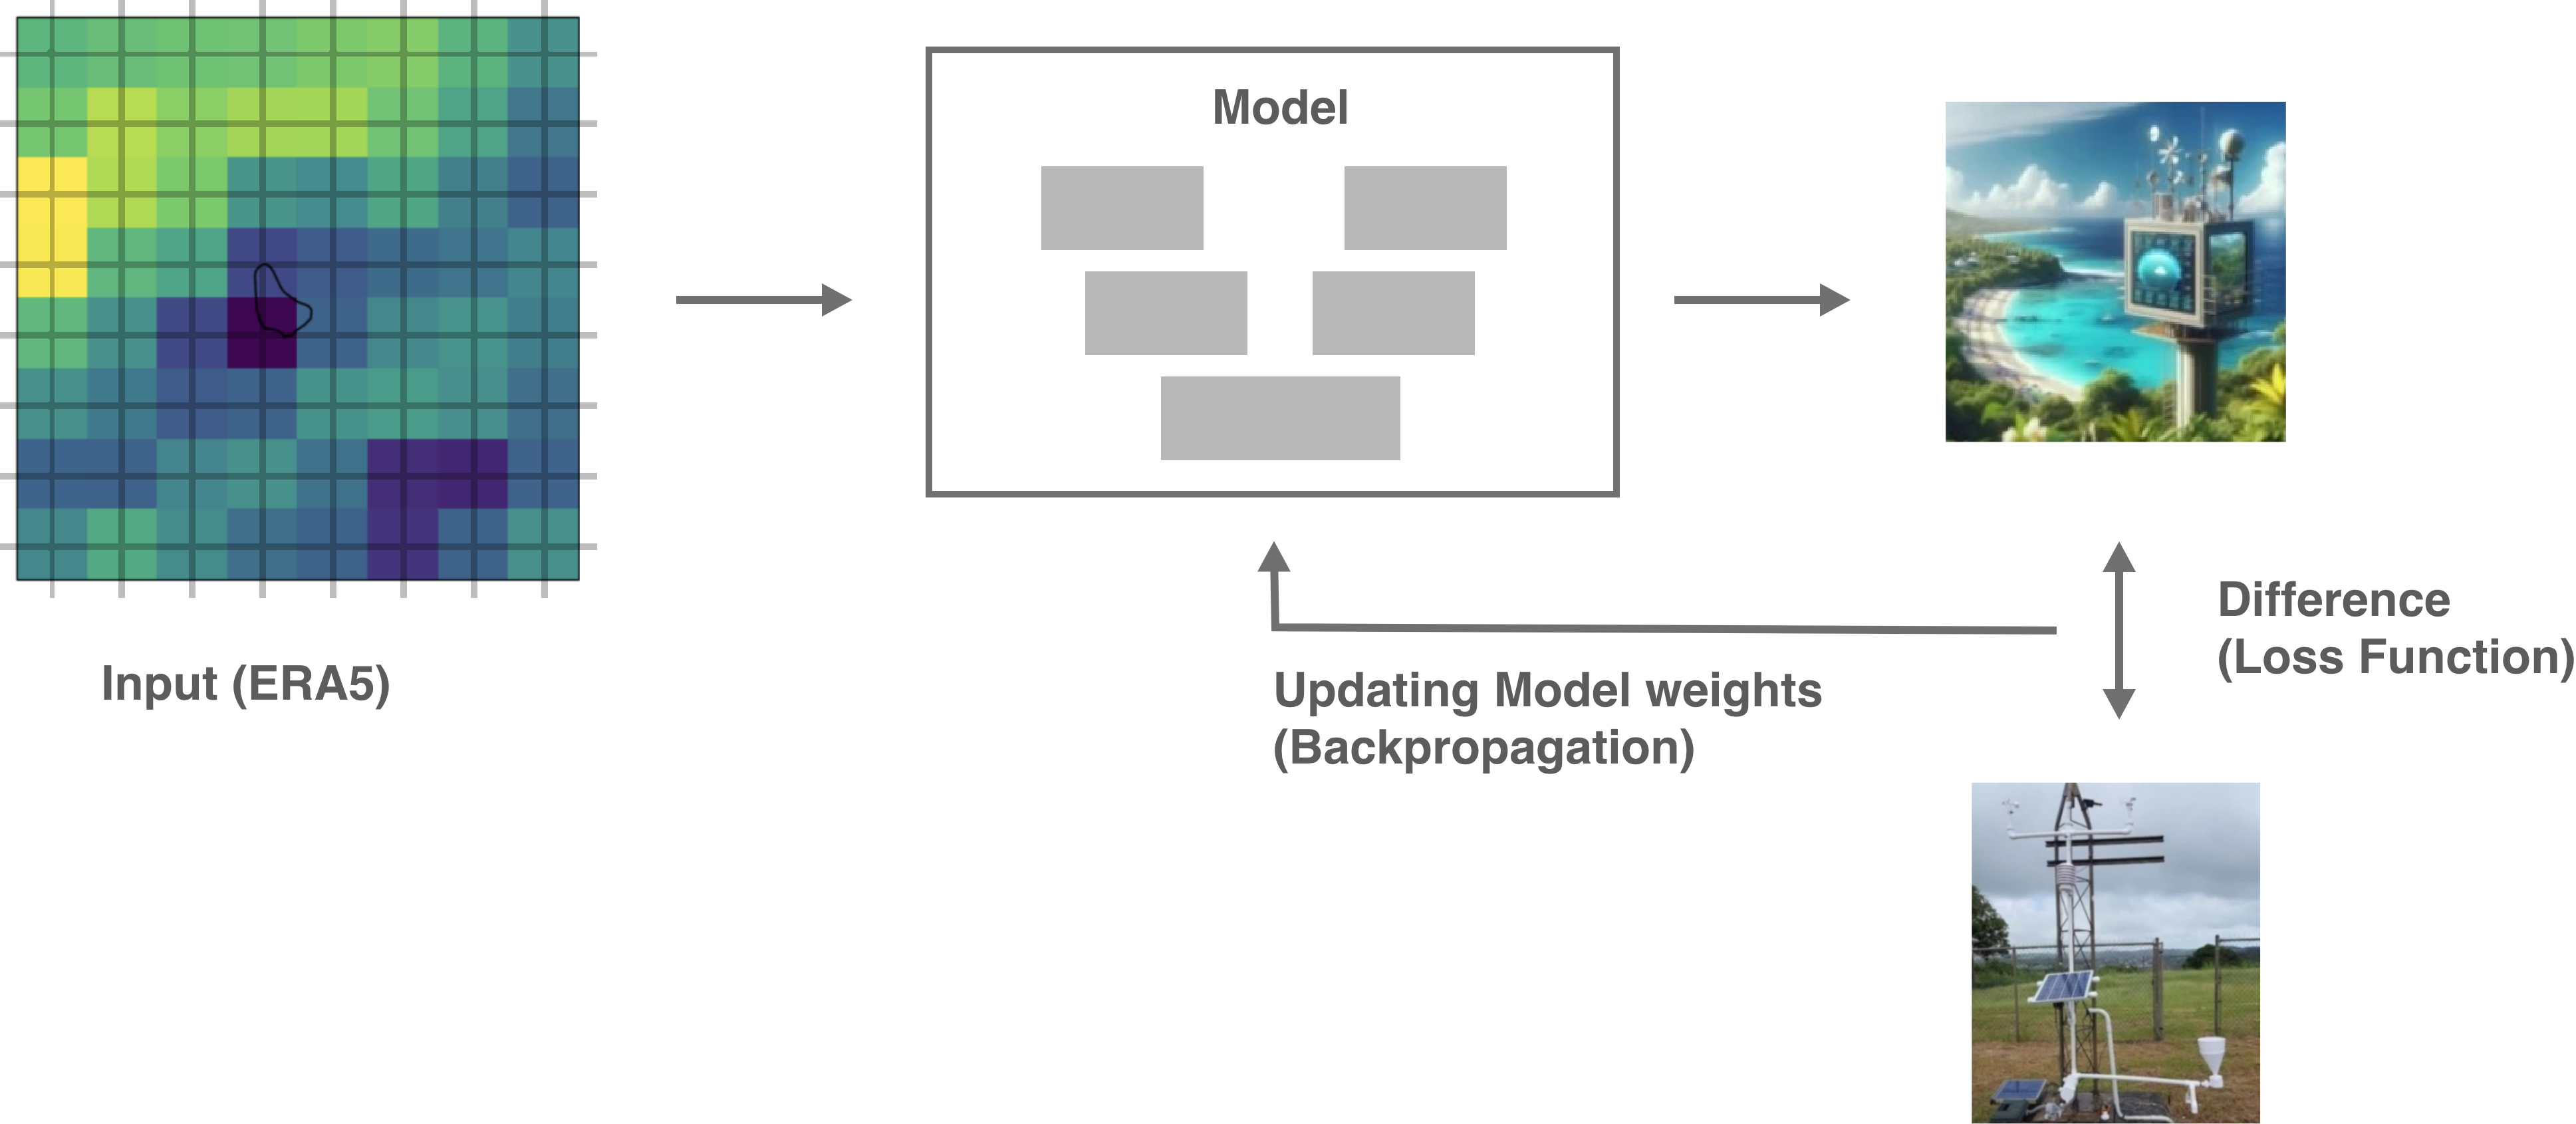
\includegraphics[width=\textwidth]{resources/images/supervised_learning.png}
    \caption{Conceptual framework using supervised learning.}
    \label{fig: supervised_learning}
\end{figure}

\begin{figure}
    \centering
    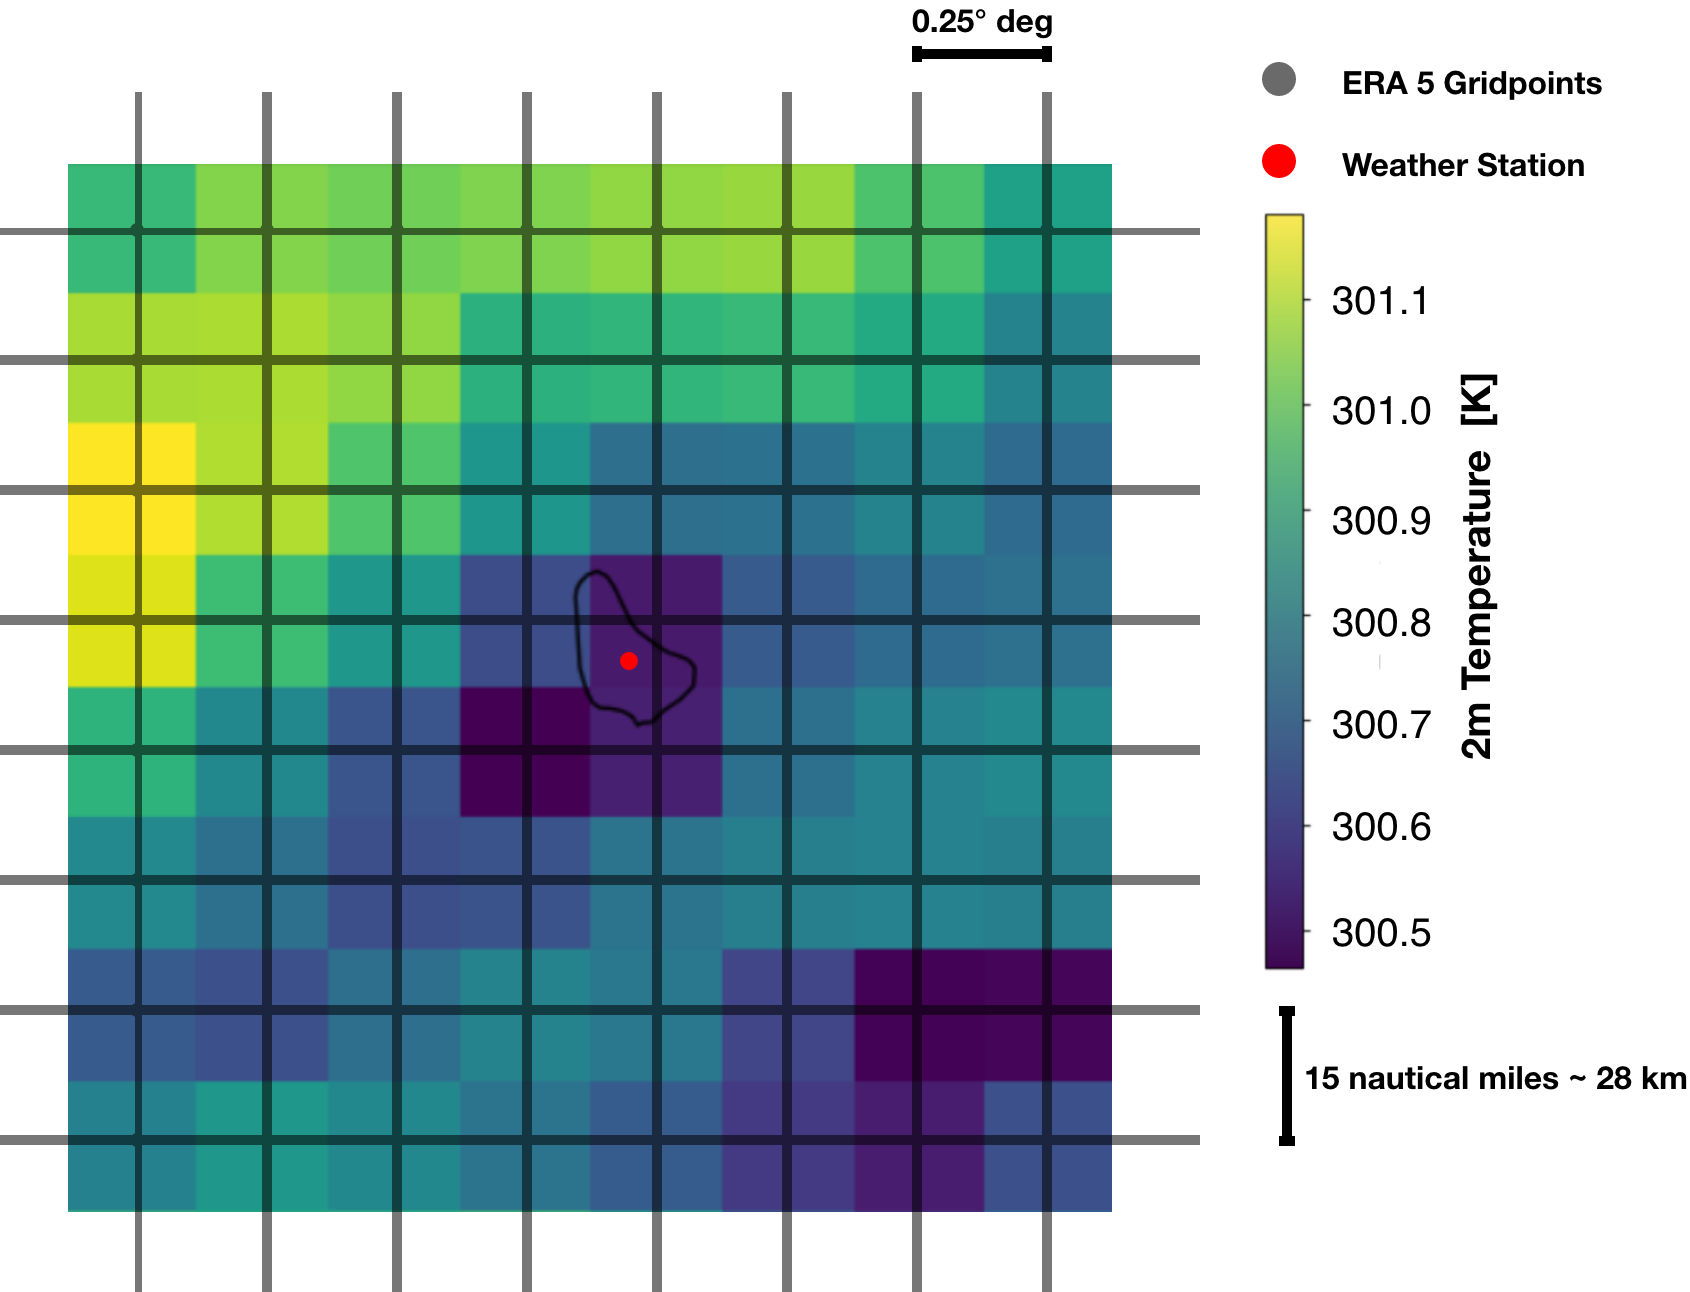
\includegraphics[width=0.9\textwidth]{resources/images/ERA5_tas_around_barbados.png}
    \caption{8x8 grid-points of ERA5 with the 2-meter temperature 
    for 2020-06-23 19:00 UTC  in the area of a weather station on Barbados.}    
    \label{fig: barbados}
\end{figure}

The conceptual framework of the proposed method is illustrated in \autoref{fig: supervised_learning}.
Applying the local patterns at the weather station location on top of ERA5 would reconstruct the temperature data at the station.
The idea is that a Convolutional Neural Network would learn to recognize the relevant patterns in a regional cutout of ERA5 data in the station area.
An example of such a cutout is shown in \autoref{fig: barbados}.
Based on the regional ERA5 data, the network would then predict the temperature at the weather station.
To illustrate with an example in what form these discrepancies can emerge:
In the case of Barbados, the grid cells of the ERA5 data all lay primarily in the ocean, meaning the diurnal cycle has a much lower amplitude than at the weather station that is located on land.
The neural network would need to learn how to detect the diurnal cycle phase based on the 64 grid points and then adjust the temperature values accordingly.
Besides this obvious difference between ERA5 and the measurements at Barbados, there are most likely many more dynamic local effects to be learned and adjusted for.

Since the ERA5 data is available globally and hourly, any weather station's missing hour could be reconstructed simply with a model that has been trained for the respective station.
A supervised learning approach will be used to train the model (see \autoref{fig: supervised_learning}).
Therefore, the model's weights will be adjusted during training so that the difference between the prediction based on an ERA5 input and the actual measurement is minimized.
The design decision to make the model based on one timestep of input for one timestep of output and not on a sequence of timesteps has the following advantages: It allows for simplicity in training, as no sequence handling is needed but simply any single timestep can be used for training.
It also allows for flexibility in application, as the model can be applied to any single timestep of ERA5 data to reconstruct the temperature at the weather station at that time.
The disadvantage is that the model cannot learn from the sequence of timesteps, meaning it cannot learn from the temporal evolution of the weather patterns.
However, that is not anticipated to be a problem because the time evolution is part of the spatial distribution of temperature in the ERA5 grid, as weather systems and the daily cycle have this implicit.
Therefore, when reconstructing missing data, the model is applied to the ERA5 data hour by hour, and the result is a series of hourly predictions that are not explained and only implicitly connected in time.

\subsection{Data Acquisition and Preprocessing}
\label{subsec: data_preprocessing}
Upon obtaining a dataset from a weather station, it is determined where temperature data is missing.
While the weather station dataset is minute-based, data could be missing only for a few minutes within an hour instead of the full hour.
This would raise the question of how many missing values are acceptable to not mark the hour as missing.
Sure is, that if all temperature values are missing during an hour, the hour is marked as missing.
The ERA5 data then needs to be cropped to the neighboring 8x8 grid cells, while centering the cutout as close to the weather station as possible.
The available longitudes and latitudes in the ERA5 model are spaced by 0.25° along the latitude and longitude from each other, when 8x8 grid cells are selected it needs to be assured that the grid points are such selected that the coordinates of the weather station are between the 4th and 5th grid point in each dimension.
After cropping the ERA5 dataset geographically, the data needs to be cut and divided along the time axis to match the weather station data, leading to two datasets: one with all the hours marked as missing and one with all the hours marked as present.
Until the model is trained, only the dataset with all the hours marked as present will be used.

As a result, we have a dataset pair of weather station measurements and ERA5 data, that are coherent in time and space.

\subsection{Training of the Convolutional Neural Network}
The next step is to train a Convolutional Neural Network (CNN); for further theoretical background on CNNs see \autoref{subsec: cnn}.
To determine after the training if and to which extent the model learned to reconstruct the missing data, the dataset pair is split again along the time axis into a pair of station with ERA5 data for training and a pair of station with ERA5 data for validation.
Thus we can later let the model reconstruct values that have actually been measured but haven't been included in the training so we then can validate how successful the reconstruction is.
With the datasets prepared, the next phase involves configuring and training the CNN for the temperature reconstruction task.
The CNN architecture is tailored to accept input in the form of 8x8 grid cells centered around the weather station's location.
Employing a supervised learning approach, the CNN is trained using pairs of hourly temperature data from the weather station and corresponding grid cell data from ERA5.
The training process iteratively feeds batches of data into the CNN, fine-tuning its parameters to minimize prediction errors and optimize accuracy in reconstructing missing temperature values.

\subsection{Validation of the trained model}
Following the training phase, the CNN's performance is evaluated using the validation set.
The model's capacity to accurately reconstruct missing temperature data at the weather station is scrutinized against ground truth values.
This evaluation step serves to gauge the CNN's proficiency in capturing intricate weather patterns and producing precise temperature estimations.
For that, the root mean squared error (RMSE) and the Pearson correlation coefficient (correlation coefficient) are calculated.
The RMSE is a measure of the differences between predicted and observed values, while the correlation coefficient quantifies the strength and direction of the linear relationship between the two datasets.
An obvious choice as a time range for the evaluation would be to cut out one complete year so that the model can be evaluated over the full range of seasons and weather conditions.

\subsection{Application for infilling}
Upon successful training and validation, the model is trained again with the measurements that have been excluded before for the benefit of validation.
After training on the complete data, the CNN can be used to fill gaps.
Fundamentally, the predictions can be made for any list of timesteps. Firstly, the needed ERA5 data, for the respective timesteps will be obtained, and secondly cropped in the same way to the geographical region as during training and then given as input to the model.
The result is a list of temperature values that are not connected in time but are the model's prediction for the temperature at the weather station at the respective time.
To predict the temperature at all those times where measurements are missing, preprocessing work can be shortened, with the available datasets already prepared in \ref{subsec: data_preprocessing}.
For the training the ERA5 dataset was already split into one with all hours marked as missing and one with all hours marked as present.
Thus, the model can directly be applied to the dataset with all hours marked as missing and then directly filled into the original measurements dataset.
Insights about the respective software implementation are given in \autoref{sec: implementation} and \autoref{sec: process_orchestration}.